
% \documentclass[manuscript]{aastex}
\documentclass[12pt,preprint]{aastex}
%\documentclass[preprint2]{aastex}
%\documentclass[aaspp4]{aastex}
%\documentclass{aastex}
%\documentclass[]{emulateapj}
%\documentclass[onecolumn]{emulateapj}

%!TEX TS-program=latex
\usepackage{amsmath}
%\usepackage{pdfsync}
%\def\snp{SN\,II-P} 
%\def\snep{SNe\,II-P} 
%\def\VmI{\hbox{$V\!-\!I$}} 
%\def\fe{\ion{Fe}{2}}
%\newcommand{\bvri}{\protect\hbox{$BV\!RI$} }

\citestyle{aa}

\begin{document}

% \slugcomment{Draft \today}
%\submitted{Draft \today} 

\title {Ay 190 Worksheet 7} 
\shorttitle{WS2}
\shortauthors{Kleiser}

\author{Io Kleiser} \affil{Caltech} \email{ikleiser@caltech.edu}

\section*{pp-Chain Nucleosynthesis}

Figures \ref{f:T_1e7}, \ref{f:T_2e7}, and \ref{f:T_3e7} show the evoluton of $^1$H and $^4$He for central temperatures of $1 \times 10^7$,  $2 \times 10^7$, and $3 \times 10^7$ K, respectively. If the main sequence lifetime of the Sun is $10^{10}$ years and there should be a remaining mass hydrogen mass fraction of 0.02, then based on these plots the temperature should be between $2 \times 10^7$ and $3 \times 10^7$ K. The actual central temperature is $1.5 \times 10^7$.

\begin{figure}[!ht]
\begin{center}
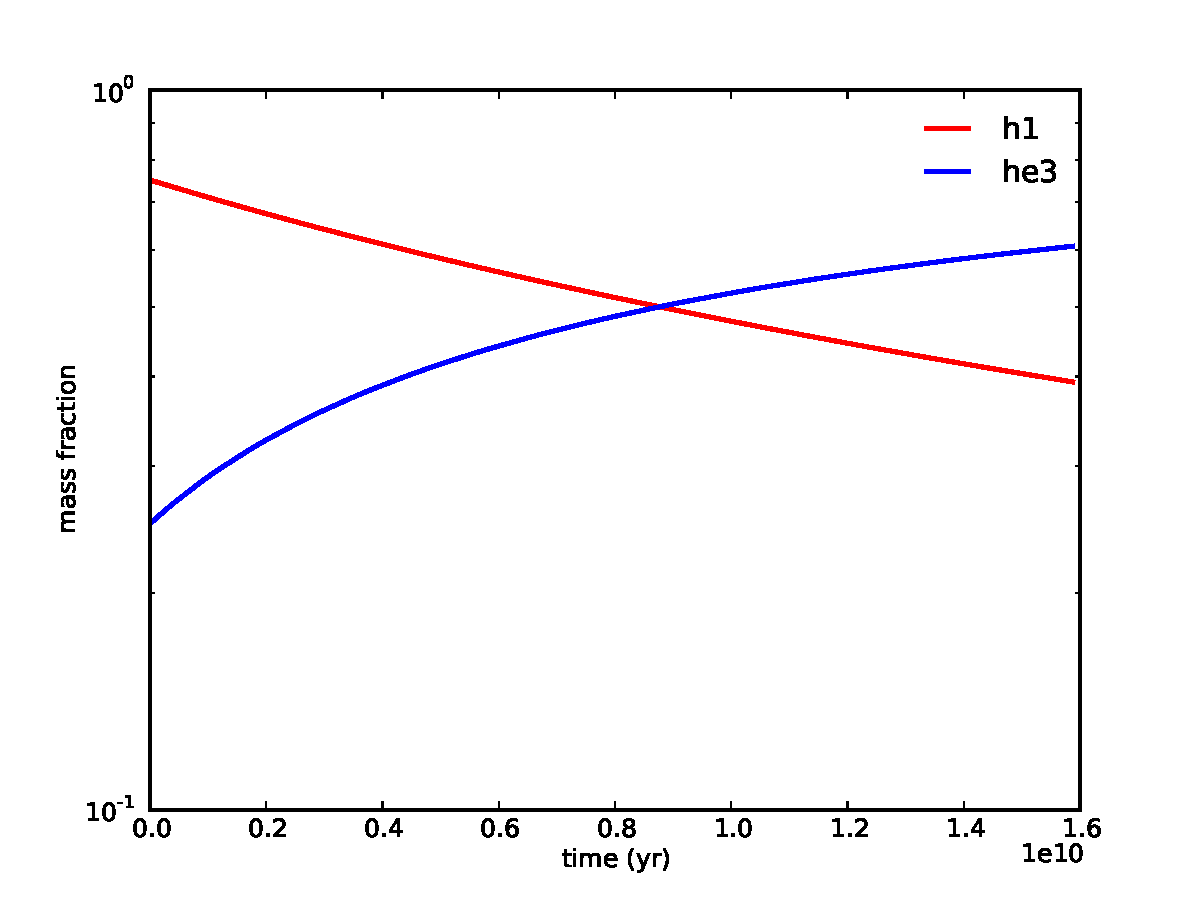
\includegraphics[width=5in]{T_1e7.pdf}
\end{center}
\caption{ \label{f:T_1e7}}
\end{figure}

\begin{figure}[!ht]
\begin{center}
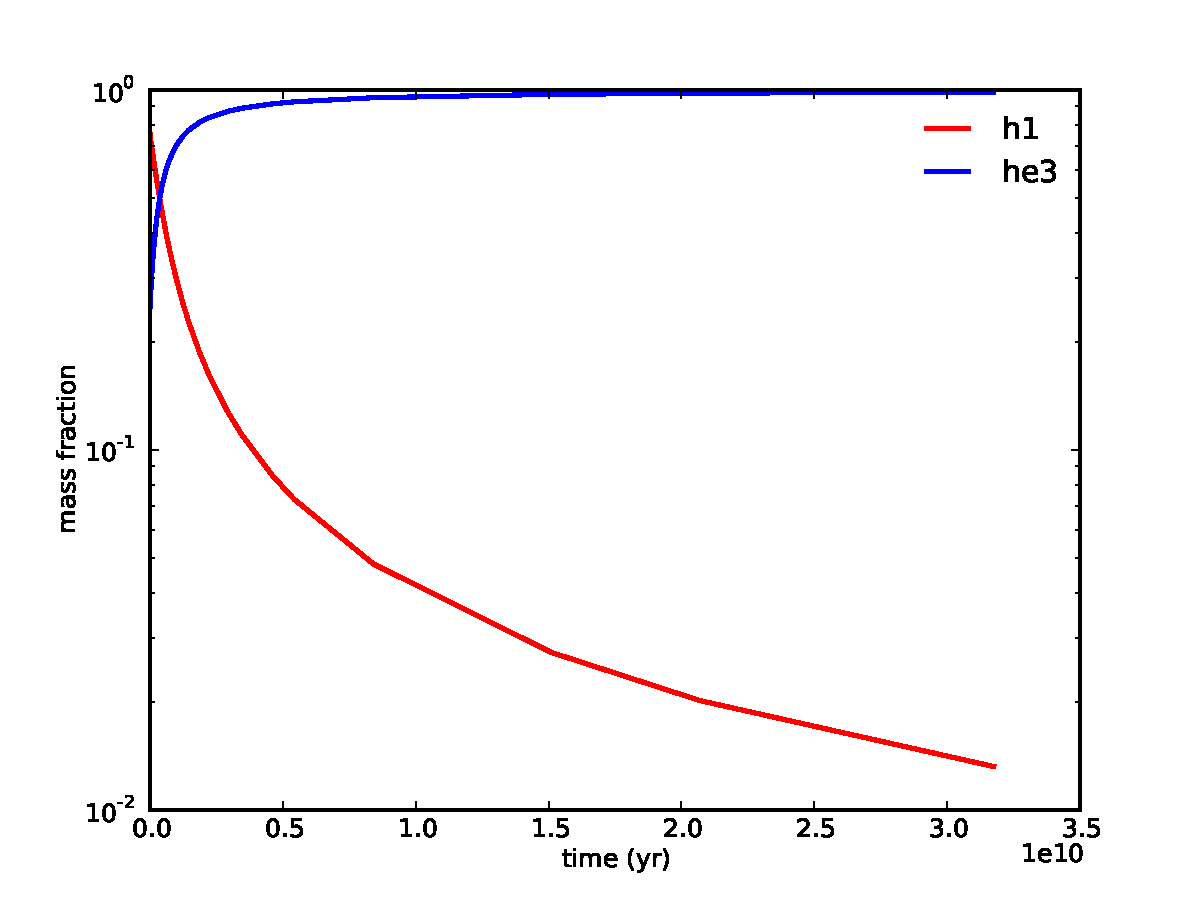
\includegraphics[width=5in]{T_2e7.pdf}
\end{center}
\caption{ \label{f:T_2e7}}
\end{figure}

\begin{figure}[!ht]
\begin{center}
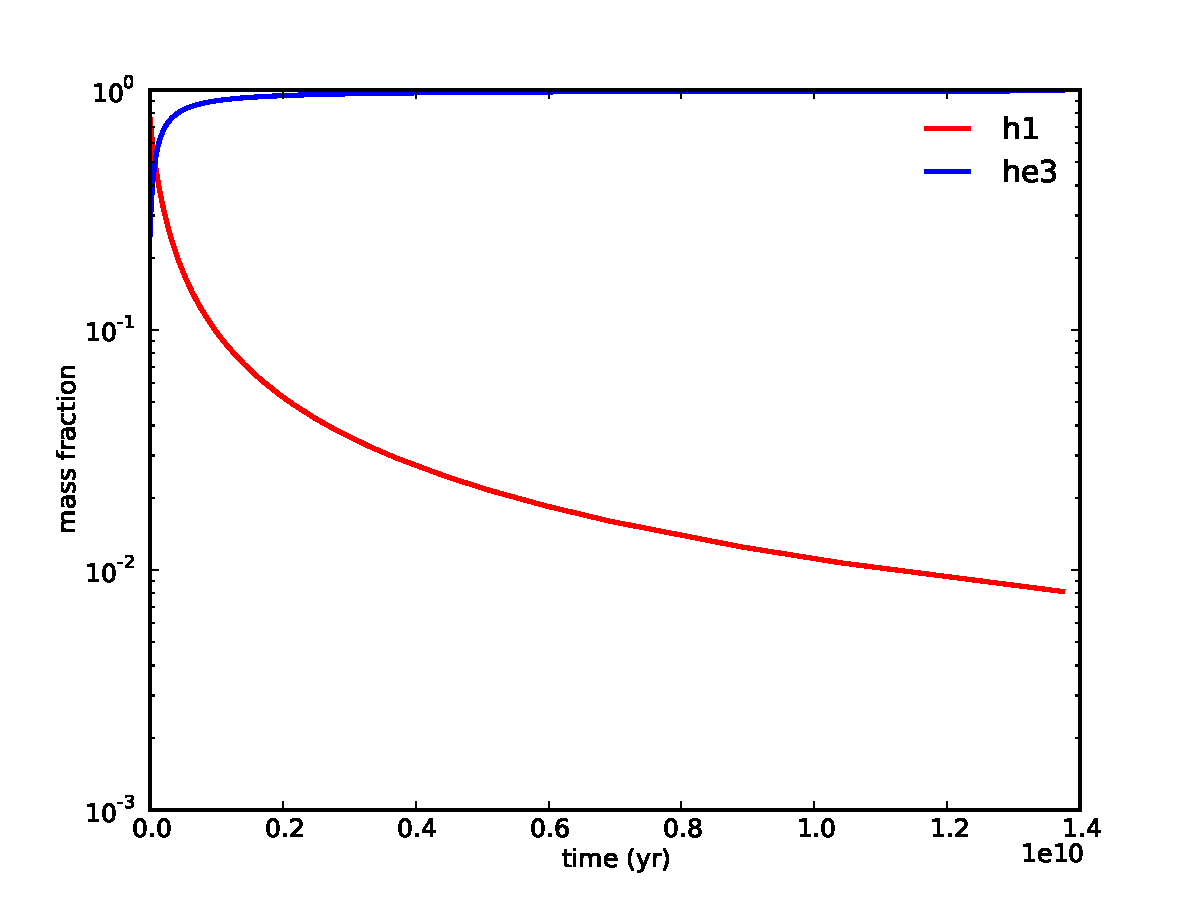
\includegraphics[width=5in]{T_3e7.pdf}
\end{center}
\caption{ \label{f:T_3e7}}
\end{figure}

The pp chain starts as follows:
\begin{equation}
^1_1{\rm H} + ^1_1{\rm H} \longrightarrow ^2_2{\rm He}
\label{eq:pp0_a}
\end{equation}
\begin{equation}
^2_2{\rm He} \longrightarrow ^2_1{\rm D} + {\rm e}^+ + \nu_{\rm e}
\label{eq:pp0_b}
\end{equation}
The combination of these two reactions becomes:
\begin{equation}
^1_1{\rm H} + ^1_1{\rm H} \longrightarrow ^2_1{\rm D} + {\rm e}^+ + \nu_{\rm e} + 0.42~{\rm MeV}
\label{eq:pp_1}
\end{equation}
We also have:
\begin{equation}
{\rm e}^- + {\rm e}^+ \longrightarrow 2\gamma + 1.02~{\rm MeV}
\label{eq:pp_2}
\end{equation}
and
\begin{equation}
^2_1{\rm D} + ^1_1{\rm H} \longrightarrow ^3_2{\rm He} + \gamma + 5.49~{\rm MeV}.
\label{eq:pp_3}
\end{equation}
Then, for the pp I branch, 
\begin{equation}
^3_2{\rm He} + ^3_2{\rm He} \longrightarrow ^4_2{\rm He} + 2^1_1{\rm H} + 12.86~{\rm MeV}.
\label{eq:pp_4}
\end{equation}

\section{Other pp-Chain Branches}

The other two branches of the pp chain start with Equations \ref{eq:pp0_a} and \ref{eq:pp0_b} (or Equation \ref{eq:pp_1}). They then proceed in different ways:

\subsection{pp II}

\begin{equation}
^3_2{\rm He} + ^4_2{\rm He} \longrightarrow ^7_4{\rm Be} + \gamma
\end{equation}
\begin{equation}
^7_4{\rm Be} + {\rm e}^- \longrightarrow ^7_3{\rm Li} + \nu_{\rm e} + (0.861~{\rm MeV},0.383~{\rm MeV})
\label{eq:ppII_2}
\end{equation}
\begin{equation}
^7_3{\rm Li} + ^1_1{\rm H} \longrightarrow 2 ^4_2{\rm He}
\end{equation}
In Equation \ref{eq:ppII_2}, the two different energies correspond to the production of lithium in either the ground state (90\% of the time) or in an excited state (10 \% of the time).

\subsection{pp III}

\begin{equation}
^3_2{\rm He} + ^4_2{\rm He} \longrightarrow ^7_4{\rm Be} + \gamma
\end{equation}
\begin{equation}
^7_4{\rm Be} + ^1_1{\rm H} \longrightarrow ^8_5{\rm Be} + \gamma
\end{equation}
\begin{equation}
^8_5{\rm Be} \longrightarrow ^8_4{\rm Be} + {\rm e}^+ + \nu_{\rm e}
\end{equation}
\begin{equation}
^8_4{\rm Be} \longrightarrow 2 ^4_2{\rm He}
\end{equation}

\section{Formulation of the pp I Reaction Network}

Let's use Equations \ref{eq:pp0_a}, \ref{eq:pp0_b}, \ref{eq:pp_2}, \ref{eq:pp_3}, and \ref{eq:pp_4}. The rate of change in number density for $^1_1{\rm H}$, $^2_2{\rm He}$, $^2_1{\rm D}$, $^3_2{\rm He}$, and $^4_2{\rm He}$ are:
\begin{equation}
\frac{dn_{\rm H}}{dt} = - n_{\rm H}^2 <\sigma v>_{\rm HH} - n_{\rm H} n_{\rm D}<\sigma v>_{\rm H D} + n_{\rm He 3}^2 <\sigma v>_{\rm He3 He3}
\label{eq:rate_1}
\end{equation}
\begin{equation}
\frac{dn_{\rm He2}}{dt} = -\lambda_{\rm He2} n_{\rm He2}
\label{eq:rate_2}
\end{equation}
\begin{equation}
\frac{dn_{\rm D}}{dt} = - n_{\rm H} n_{\rm D} <\sigma v>_{\rm HD} + \lambda_{\rm He2} n_{\rm He2}
\label{eq:rate_3}
\end{equation}
\begin{equation}
\frac{dn_{\rm He3}}{dt} = n_{\rm H} n_{\rm D} <\sigma v>_{\rm HD} - n_{\rm He3}^2 <\sigma v>_{\rm He3He3} 
\label{eq:rate_4}
\end{equation}
\begin{equation}
\frac{dn_{\rm He4}}{dt} = n_{\rm He3}^2 <\sigma v>_{\rm He3He3} 
\label{eq:rate_5}
\end{equation}

We can use (from the notes)
\begin{equation}
\frac{dn_i}{dt} = \rho N_A \frac{dY_i}{dt} + N_A Y_i \frac{d \rho}{dt} = \rho N_A \frac{dY_i}{dt}
\end{equation}
if $d\rho/dt = 0$. Then we can rewrite these equations as

\begin{equation}
f_{\rm H} = \frac{dY_{\rm H}}{dt} = -N_A \rho \lambda_{\rm HH} Y_{\rm H}^2 - N_A \rho \lambda_{\rm HD}Y_{\rm H}Y_{\rm D} + N_A \rho \lambda_{\rm He3He3} Y_{\rm He3}^2 
\end{equation}
\begin{equation}
f_{\rm He2} = \frac{dY_{\rm He2}}{dt} = -\lambda_{\rm He2}n_{\rm He2}
\end{equation}
\begin{equation}
f_{\rm D} = \frac{dY_{\rm D}}{dt} = N_A \rho \lambda_{\rm HD}Y_{\rm H}Y_{\rm D} + \lambda_{\rm He2}n_{\rm He2}
\end{equation}
\begin{equation}
f_{\rm He2} = \frac{dY_{\rm He2}}{dt} =N_A \rho \lambda_{\rm HD}Y_{\rm H}Y_{\rm D} - N_A \rho \lambda_{\rm He3He3} Y_{\rm He3}^2
\end{equation}
\begin{equation}
f_{\rm He4} = \frac{dY_{\rm He4}}{dt} = N_A \rho \lambda_{\rm He3He3} Y_{\rm He3}^2
\end{equation}

Following the derivation in the notes, we can set up a system of equations
\begin{equation}
\Delta_i - \sum_{j}\frac{df_i}{dY_j}\Delta_j \Delta t = f_i(t)\Delta t
\end{equation}
where $\Delta_i = Y_i(t + \Delta t) - Y_i(t)$.

%\bibliographystyle{apj2} 
%\bibliography{gal}

%\bibliography
\end{document}
